\chapter{From edges to contours} % - Current State-of-the-Art}
\label{Chapter3}
\section{gPb-owt-ucm algorithm pipeline}
The gPb algorithm utilises local cues - colour, brightness and texture to build features. Those are then globalised using spectral clustering. Multiple-scale approach gives competitive edge detection results.

it is straightforward to close contours using a watershed operation (basic morphological operation)

watershed contours is a binary image (c.f. edge map) indicating the highest level of recall

\begin{figure}[ht!]
\centering
 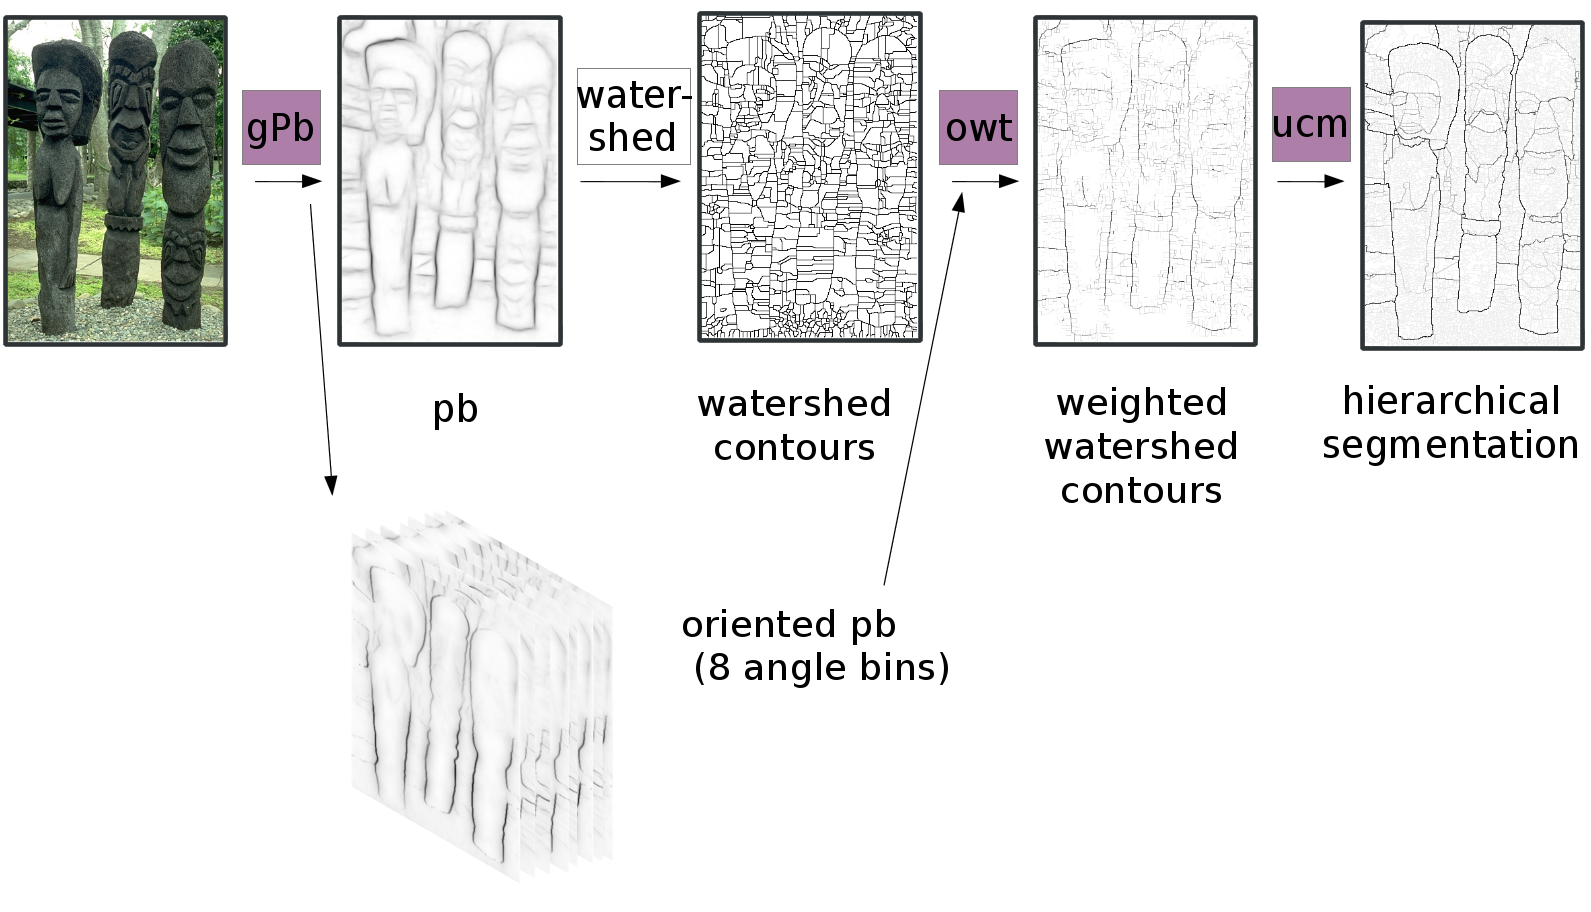
\includegraphics[width=1\textwidth]{images/gPb-OWT-UCM/gPb-OWT-UCM_pipeline.png}
\caption{gPb-OWT-UCM algorithm. We have expanded the pipeline to explicitly include the ``watershed transform'' operation and its output - watershed contours.}
\label{fig:gPb-OWT-UCM-pipeline}
\end{figure}

\subsection{Quantised oriented probability of boundary}
\subsection{Weighted watershed}
\section{Limitations of quantisation} % or drawbacks, don't say 'flaws'